\documentclass[a4paper, 10pt, final, garamond]{book}
\usepackage{cours-preambule}

\makeatletter
\renewcommand{\@chapapp}{Devoir surveill\'e -- num\'ero}
\makeatother

\toggletrue{corrige}

\begin{document}
\setcounter{chapter}{3}

\def\lspace{25}

\chapter{Commentaires sur le DS \oldno4}

\section{Commentaires généraux}
\subsection{Appréciation globale}
Champagne~!! Un super DS juste avant les vacances d'hiver. En voilà un beau
cadeau. Moyenne à 11/20, 110 points bonus, 18 points malus.
\smallbreak
Votre travail porte ses fruits, et vous récupérez bien du catastrophique DS02.
L'ensemble de la classe s'est amélioré, et les connaissances générales sur la
résonance et la cinétique sont globalement acquises. Bravo à vous. Maintenez ce
cap pour le second semestre~!

\begin{center}
	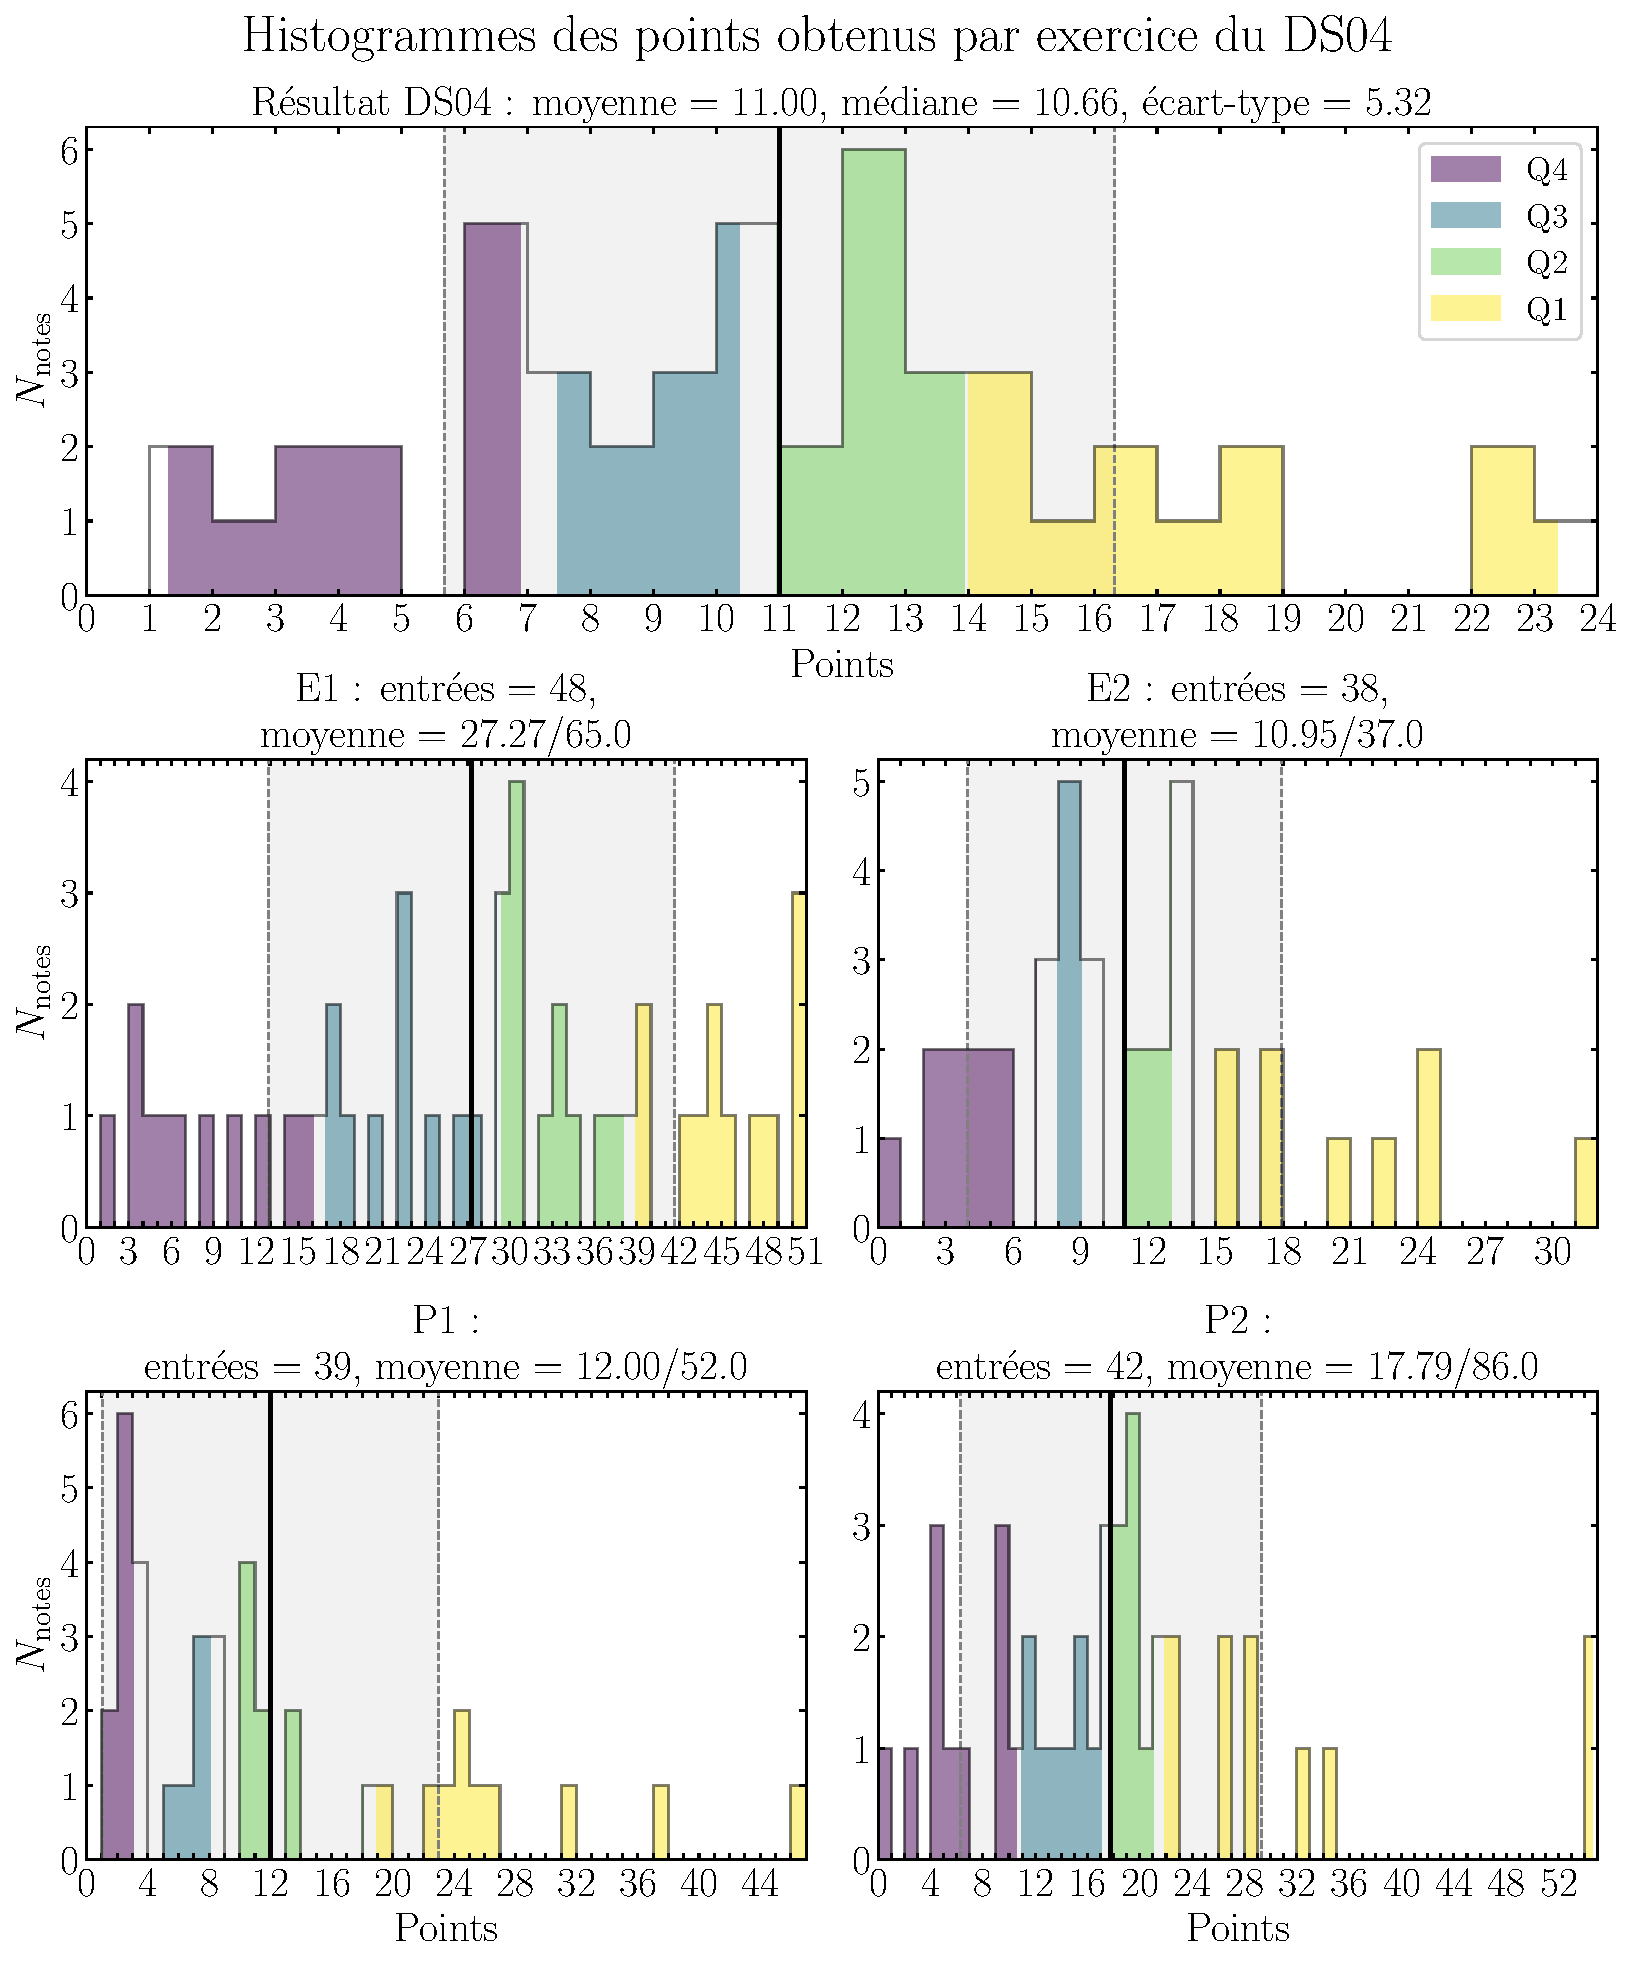
\includegraphics[width=.8\linewidth]{DS04_hist_all}
	\caption{Graphique des résultats}
\end{center}

\subsection{Sur la forme}
Numérotez les \textbf{copies} et pas les pages, et numérotez les copies en
donnant le nombre de copie maximal~! Copie 1 $\Ra$ et alors~? Copie 1/2 $\Ra$ il
existe une autre copie. À savoir et à ne pas manquer.
\smallbreak
\textbf{Indiquez quand il y a des questions de l'autre côté d'une page
	pratiquement vide~!!} Un petit «~TSVP~» pour «~tournez s'il vous plaît~» fait
toute une différence sur le sentiment que vous faites un effort à alléger le
travail de correction, et ça ira très loin dans l'appréciation générale de votre
copie.
\smallbreak
Encore de bons efforts sur les commentaires antérieurs. Par contre, essayez de
vous \textbf{approprier} les commentaires. Je vous demanderai de ne \textbf{pas
	simplement me citer} mais de \textbf{reformuler avec vos mots} les points
importants que j'énonce. J'augmenterai les points bonus en conséquence. Si c'est
bien fait, ça pourra être vraiment bien récompensé.
\begin{tcn}(exem)<lftt>{Exemple de commentaire vraiment utile ou non}
	\begin{itemize}
		\item Premier exemple, commentaire DS04 2023~:
		      \begin{itemize}
			      \item Citation simple~: «~il faut connaître la différence entre
			            méthode intégrale/différentielle~»~: \pt{1} bonus
			            actuellement.
			      \item Reformulation~: «~méthode différentielle = on trace $\ln (v)$
			            et la pente est l'ordre partiel~; méthode intégrale = on
			            travaille sur $[\ce{A}](t)$ et le résultat dépend de l'ordre
			            (0, 1 ou 2)~»~: \pt{4} facilement~!
		      \end{itemize}
		\item Second exemple, commentaire DS03 2024~:
		      \begin{itemize}
			      \item «~$\xi\ind{eq} \neq \xi\ind{max}$ même en conditions
			            stœchiométriques~» \pt{1} ou peut-être \pt{2}
			      \item «~les conditions stœchiométriques portent sur les conditions
			            \textbf{initiales} de proportionnalité entre les réactifs,
			            mais ne dit rien sur l'état final~: il n'est pas forcément
			            maximal~!»~: \pt{4} facile~!
		      \end{itemize}
	\end{itemize}
\end{tcn}

Le but des commentaires n'est pas que vous soyez des scribes, mais que vous
preniez le temps de vous poser des questions \textbf{et cherchiez les réponses}
en lisant mes commentaires.
\smallbreak
Enfin, \textbf{n'en faites pas trop non plus}, une ou deux phrases suffisent, ne
refaites pas de démonstration dans le cadre remarque… Et vous pouvez continuer à
ne faire que citer des portions des commentaires, je ne vous pénaliserai pas,
mais je veux que vous commenciez à faire plus que ça.

\subsection{Commentaires principaux et récurrents}
Revoyez la méthode différentielle pour la cinétique chimique. Concentrez-vous
bien sur les calculs fondamentaux en résonance. Mes conseils basés sur
l'interrogation de lundi dernier (ainsi que les commentaires du DS04 de 2023)
ont, semble-t-il, porté leurs fruits. À vous d'essayer de faire le même résumé
et le même «~dézoom~» sur les chapitres suivants~!

\setcounter{section}{0}
\section[65]"E"{Étude d'un circuit RLC parallèle}
\begin{enumerate}
	\item[n]{3} % Q1
	      Ça ne sert à rien d'ajouter les admittances 2 par 2~! Si vous avez 3
	      impédances en série, vous faites $\Zu = \Zu_1+\Zu_2+\Zu_3$. Pour 3
	      impédances en parallèle, $\Yu = \Yu_1+\Yu_2+\Yu_3$~! Attention à
	      l'homogénéité… Pas trop de crimes sur cette question, c'est bien~!
	\item[n]{5} % Q2
	      Ne sautez pas sur un pont diviseur de tension quand vous avec un circuit
	      avec une seule impédance équivalente. Choisissez votre méthode en
	      fonction de ce que vous avez.
	      \smallbreak
	      Répondez à la question~: donnez $\w_0$ et pas $\w_0{}^2$.
	      \smallbreak
	      \textbf{Identifiez}. Gros problèmes d'identification…
	\item[n]{2} % Q3
	      Indiquez que vous prenez le module. N'oubliez pas la racine carrée~!
	\item[n]{8} % Q4
	      La résonance est un \textbf{phénomène physique}, donc ça n'est
	      \textit{ni une résonance ni une amplitude}. Les formulations du style
	      «~la résonance c'est la fréquence maximale~» ou «~c'est l'amplitude
	      maximale~» ne font pas sens. \textbf{À la fréquence de résonance}, il y
	      a un \textbf{maximum d'amplitude} réelle.
	      \smallbreak
	      N'oubliez pas \textbf{pour $\boxed{\w \neq 0~;\infty}$}~! Personne n'a
	      eu la totalité des points sur cette question.
	\item[n]{8} % Q5
	      La bande passante c'est une différence de \textbf{pulsations} (ou
	      fréquences), donc vous ne pouvez pas écrire
	      \[
		      \Delta{\w} = \frac{U\ind{max}}{\sqrt{2}}
		      \quad \red{\circled{$-$H}}
	      \]
	      Il faut mettre les trinômes \textbf{sous forme de trinôme}~!
	      \[
		      \boxed{a x^2 + b x + c = 0}
		      \qMath{et pas}
		      \cancel{ax + \frac{b}{x} + c = 0}
	      \]
	\item[n]{7} % Q6
	      \textbf{Ne confondez pas équivalent asymptotique et limite~!}
	      { \Large
		      \[
			      \Sim_{x \to 0} \neq \opto{}{x \to 0}
		      \]
	      }
	      Tracez, bon sang~!
	\item[n]{6} % Q7
	      \leavevmode\vspace*{-15pt}\relax
	      {\Large
		      \[
			      \phi(x) = \arg*{\boxed{\xul{U_0}}}
			      \qMath{et pas}
			      \phi(x) = \arg*{\abs{\xul{U_0}}}
		      \]
	      }
	      Sinon c'est l'argument d'un réel positif, c'est toujours nul…
	      \[
		      \boxed{\f \neq \phi \neq \Phi \neq \varnothing}
		      \quad \text{!}
	      \]
	      \smallbreak
	      On peut toujours composer par $\tan(\cdot)$. C'est pour composer par
	      $\boxed{\arctan(\cdot)}$ qu'il faut faire attention~!
	\item[n]{5} % Q8
	      RAS.
	\item[n]{4} % Q9
	      Horrible, horrible représentation du courant $\eta$ sur le schéma. Il a
	      échappé à ma vigilance. Je vous présente mes excuses pour vos yeux
	      meurtris.
	      \smallbreak
	      Très mal gérée, 47\% de 1 point uniquement. Il faut revoir les notions
	      de masse dans un circuit, et comment un représente la tension que lit un
	      oscilloscope.
	\item[n]{5} % Q10
	      Bof.
	\item[n]{5} % Q11
	      Bof. L'amplitude se lit sur le graphique~!
	\item[n]{2} % Q12 
	      Attention aux unités.
\end{enumerate}

\section[37]"E"{Monoxyde et dioxyde d'azote}
\begin{enumerate}
	\item[n]{6} % Q1
	      Il y a 4 fois plus de diazote que d'oxygène dans l'air. Cf.\ premier
	      exercice de TDTM2\_app.
	\item[n]{11} % Q2
	      Il faut voir que la réaction était quasi-nulle~! Réentraînez-vous sur
	      les cas classiques de TM, quasi-totale ou quasi-nulle. Vous ne pouvez
	      pas négliger quelque chose de petit devant rien d'autre~:
	      $n_{\ce{NO},\eql}$ est certes sans doute très petit, mais ça ne peut pas
	      être négligé~! Il faut quand même du produit, sinon $Q_r = 0$.
	\item[n]{7} % Q3
	      Constante de réaction $K^\circ \neq k$ constante de vitesse… Retour sur
	      les confusions entre favorisé et sens de réaction. N'oubliez
	      pas la puissance sur la concentration initiale dans $k\ind{app}$.
	      \smallbreak
	      Trop de confusions sur quelle concentration ne varie pas. C'est l'excès
	      qui voit sa concentration stagner.
	\item[n]{4} % Q4
	      Vous êtes tombé-es dans le panneau. On trace $\ln (v)$, ça na
	      \textbf{rien à voir} avec $\ln c(t)$. \textbf{La méthode différentielle}
	      ($\ln (v)$) n'est \textbf{pas la méthode intégrale} (régressions
	      variées).
	\item[n]{4} % Q5
	      Les vitesses $v_1$ et $v_2$ sont différentes~! Ça se voit avec les
	      régressions. Ne partez pas d'une égalité clairement fausse.
	\item[n]{2} % Q6
	      Les proportions stœchiométriques n'ont \textbf{RÀV} avec le fait que les
	      ordres partiels soient ou non égaux aux coefficients stœchiométriques.
	\item[n]{3} % Q7
	      RAS.
\end{enumerate}

\setcounter{section}{0}
\section[52]"P"{Suivi cinétique de la formation du dibrome}
\begin{enumerate}
	\item[n]{2} % Q1
	      Bien.
	\item[n]{8} % Q2
	      Faire un schéma pour montrer que chaque concentration est divisée par
	      2~! Cf.\ TP11… \textbf{Une seule personne a fait la dilution}~!
	      \smallbreak
	      Faites des tableaux d'avancement~!
	\item[n]{6} % Q3
	      Bien.
	\item[n]{13} % Q4
	      Globalement correct, mais pour une question aussi banale c'est dommage
	      qu'elle soit si peu réussie. Personne n'a eu la totalité des points.
	\item[n]{9} % Q5
	      Oui c'est moi qui ai rajouté cette question :-).
	      \smallbreak
	      \textbf{Tracez les données avec des croix}~! On se moque de la droite
	      toute seule.
	      \smallbreak
	      \textbf{N'invoquez pas le coefficient de corrélation} pour
	      justifier votre régression. Il faut que la droite passe par les points.
	      \textbf{Les coefficients directeurs et ordonnées à l'origine ont une
		      unité}~!
	\item[n]{2} % Q6
	      $t_{1/2}$ se trouvait directement dans le tableau.
	\item[n]{9} % Q7
	      Très peu traitée.
	\item[n]{3} % Q8
	      RAS.
\end{enumerate}

\section[86]"P"{Résonance d'un verre}
\begin{enumerate}
	\item[n]{5} % Q1
	      Faites un effort sur les chiffres significatifs sur votre lecture… Sinon
	      bien dans l'ensemble.
	\item[n]{10} % Q2
	      Encore une fois, c'est $\ux$ et pas $\vv{x}$~!!
	      \smallbreak
	      Décomposez entièrement les forces sur les vecteurs de base $\ux$ et
	      $\uy$.
	      \smallbreak
	      \textbf{N'inventez pas des conditions initiales} si elles ne sont pas
	      données.
	      \smallbreak
	      Lisez bien l'énoncé~: $\ell_0 = 0$~! Même pas besoin de changement de
	      variable, $x(t)$ c'est déjà $\ell(t)$.
	      \smallbreak
	      Un axe c'est une droite, $Ox$ par exemple, mais $Ox$ a l'unité d'une
	      distance~; un vecteur de base c'est $\ux$, qui est \textbf{u}nitaire,
	      pas d'unité. Donc $\dcancel{\vv{Ox}}$~!
	      \smallbreak
	      \textbf{Faites un schéma~!}
	\item[n]{5} % Q3
	      \leavevmode\vspace*{-15pt}\relax
	      \begin{itemize}
		      \item Écrivez le PFD en version \textbf{vectorielle} avant toute
		            potentielle écriture en colonnes.
		      \item Quand vous \textbf{projetez} sur $\ux$, il ne reste \textbf{que
			            des scalaires}~! Vous ne pouvez pas écrire
		            \begin{gather*}
			            \beforetext{Sur $\ux$}
			            \vv{f} + \vv{F_r} = m \af
		            \end{gather*}
		            La relation vectorielle n'est vrai que pour la somme de tous les
		            vecteurs, vous ne pouvez pas extraire une partie de l'équation.
		            C'est comme si vous écriviez
		            \begin{gather*}
			            a+b = c+d
			            \\\beforetext{donc j'extrait}
			            b = d
		            \end{gather*}
		      \item Identifiez $Q$ et $\w_0$~!
	      \end{itemize}
	\item[n]{3} % Q4
	      $\w_0$ pulsation propre = pulsation naturelle du système s'il n'y avait
	      \textbf{pas de frottements} (oscillateur harmonique), sinon c'est $\W
		      \neq \w_0$.
	\item[n]{9} % Q5
	      Frottements faibles $\neq$ frottements nuls~! Frottements faibles $\Ra Q
		      \gg 1$~! Il faut pas oublier comment résoudre le second ordre… décevant
	      à cet égard.
	\item[n]{4} % Q6
	      Très peu traitée, mais très bien quand c'est fait.
	\item{}[Q7-9] % Q7
	      Saute-mouton général.
	      % \item[n]{2} % Q8
	      % \item[n]{5} % Q9
	      \setcounter{enumi}{9}
	\item[n]{4} % Q10
	      Très mal faite. Revoyez l'origine du fait qu'on cherche une solution
	      sinusoïdale~: on considère que la solution homogène, qui tend vers 0,
	      est négligeable devant la solution particulière, et on cherche $x_p(t)$
	      de la forme de l'entrée, à la même pulsation.
	\item[n]{2} % Q11
	      Bof en vrai.
	\item[n]{4} % Q12
	      Très peu réussi. Il y a beaucoup de résonance en mécanique, il faut
	      savoir
	      «~créer~» la forme demandée en factorisant par $\w_0{}^2$.
	\item[n]{3} % Q13
	      Bien.
	\item[n]{10} % Q14
	      3 rares tentatives qui valaient le coup, sinon vous avez esquivé ce
	      calcul~! C'est le deuxième calcul à savoir faire du chapitre… c'est
	      dommage. Reprenez-le. Dans la version du corrigé, j'ai fait apparaître
	      que le minimum, s'il n'est pas en $x_r = 1$, est forcément en $x = 1$,
	      en
	      n'introduisant \textbf{pas} de $U = u^2$.
	\item[n]{2} % Q15
	      RAS.
	\item[n]{2} % Q16
	      RAS.
	\item[n]{7} % Q17
	      Rares tentatives.
	\item[n]{5} % Q18
	      RAS.
\end{enumerate}

\end{document}
